

\subsection{General interface}

\paragraph{Preliminary steps}
Once the GA3 module opened, other windows cannot be opened, therefore
\begin{itemize}
    \item you will need to open the image you want to work with first,
    \item it is convenient to open the LUT tools first (\keys{\ctrl+\Alt+L}).
\end{itemize}
To access the GA3 interface, you can either:
\begin{itemize}
    \item use the menu \menu{Image>New GA3 recipe\dots},
    \item use the menu \menu{Image>Analysis Explorer\dots} to open the analysis exporter and then click on \menu{Create New},
    \item right-click on the background of the interface, select \menu{Analysis Controls>Analysis Explorer} to open the analysis explorer and then click on \menu{Create New}.
\end{itemize}

\paragraph{Loading and saving recipes}

\begin{itemize}
    \item Use \menu{Save} or \menu{Save As} to save the recipe in the local database. It will be then listed in the Analysis Explorer.
    \item Use your name as a prefix so that we can contact you if the database needs to be cleared.
    \item Use \menu{Export} to export the recipe in a folder of your choice. This recipe can then be reloaded on another computer. It is good practice to have a copy of the recipes in that way.
    \item Use \menu{Import} to reload an exported recipe. 
\end{itemize}

\paragraph{Recipes}
\begin{figure}
    \centering \small
    \begin{tikzpicture}
        \node at (0,0) {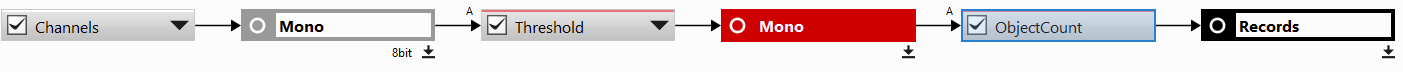
\includegraphics[width=0.75\textwidth]{artwork/simple-workflow.png}};
        % \draw[gray,very thin,step=1] (-5,-1) grid (5,1);
        \node (a) at (-5,-0.5){color};
        \node (b) at (-2,-0.5) {action};
        \node (c) at (0,-0.5) {binary};
        \node (d) at (4,-0.5) {table};
        \draw[->] (a) -| (-4,-0.2); 
        \draw[->] (b) -| (-1,-0.2); 
        \draw[->] (c) -| (1,-0.2); 
        \draw[->] (d) -| (5,-0.2); 
    \end{tikzpicture}
    \caption{A simple workflow with three kinds of nodes.}
    \label{fig:nodes}
\end{figure}

Recipes describe a workflow as a graph. The graph is composed of 4 types of nodes (See Fig.~\ref{fig:nodes}):
\begin{enumerate}\setlength\itemsep{0em}
    \item color: original or processed grayscale images
    \item action: processing steps on images, binary or tables
    \item binary: masks and labels
    \item results: tables with measurement results 
\end{enumerate}

To add an action, drag the new element to the previous one to automatically create a connection and keep the elements organized.

\paragraph{Storing results}

Saving of channels and binary layers can be enabled case by case using a right click on the layer. 

\subsection{Tips}
\begin{itemize}
    \item Use \keys{\Alt+\arrowkeyup} / \keys{\Alt+\arrowkeydown}  to increase / decrease the opacity of the binaries.
    \item To look for a module, use the search bar at the top.
    \item Right-click on the image and find image information for pixel to micron conversion.
    \item Click on the question mark on each operation (top left) for more information if needed.
\end{itemize}

\subsection{Basic image processing concepts}

\paragraph{Image} An image is any array (table) of regularly sampled intensity value. The values can range between $0$ and $2^8 = 255$ for 8-bit images or between $0$ and $2^{16}=65635$ for 16 bit images. Figure~\ref{fig:median} displays an image as graylevel and intensities values.

\paragraph{Threshold} Threshold is the simplest form of image segmentation. At each location of the image, a decision is taken to classify this point as foreground or background. In GA3, thresholds are followed by other operations such as smoothing, cleaning, connected component labelling, size filtering,\dots

\paragraph{Median filter} The median filter is creating a new image where each pixel is computed as the median value of the pixels in a neighborhood of this pixel (See Figure~\ref{fig:median}).


\begin{figure}\centering
    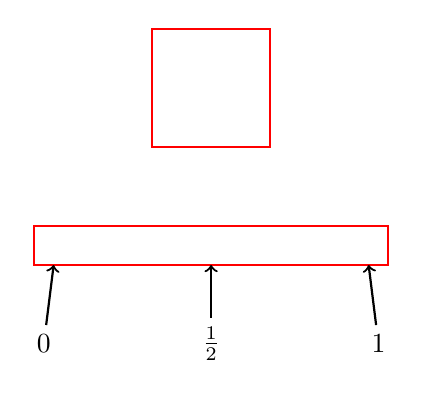
\begin{tikzpicture}[scale=0.5]
    \begin{scope}
        \def\pixels{{10,5,6,2,9},{8,5,2,4,8},{4,8,6,3,1},{2,9,7,10,3},{3,6,6,2,9}}
        \showpixelsvalue{\pixels}{0}{10}
        \draw[red,thick] (2,2) rectangle +(3,3);
    \end{scope}
    \begin{scope}[yshift=-2cm,xshift=-2cm]
        \def\pixels{{2,3,4,5,6,7,8,9,10}} 
        \showpixelsvalue{\pixels}{0}{10}
        \draw[red,thick] (1,1) rectangle +(9,1);
        \draw (1.25,-1) node {$0$} edge[->,thick] (1.5,1);
        \draw (5.5,-1) node {$\frac{1}{2}$} edge[->,thick] (5.5,1);
        \draw (9.75,-1) node {$1$} edge[->,thick] (9.5,1);
    \end{scope}
    \end{tikzpicture}
    \caption{Values in a $3 \times 3$ neighborhood are ordered to define a median (rank 1/2)
    filter. The intensity corresponding to the median value is stored in a new image.}
    \label{fig:median}
\end{figure}

\paragraph{Rolling ball} Rolling ball is used for correcting shading and non-even background. It works by subtracting a background image estimated by dilating and eroding the image.

\begin{figure}\centering
    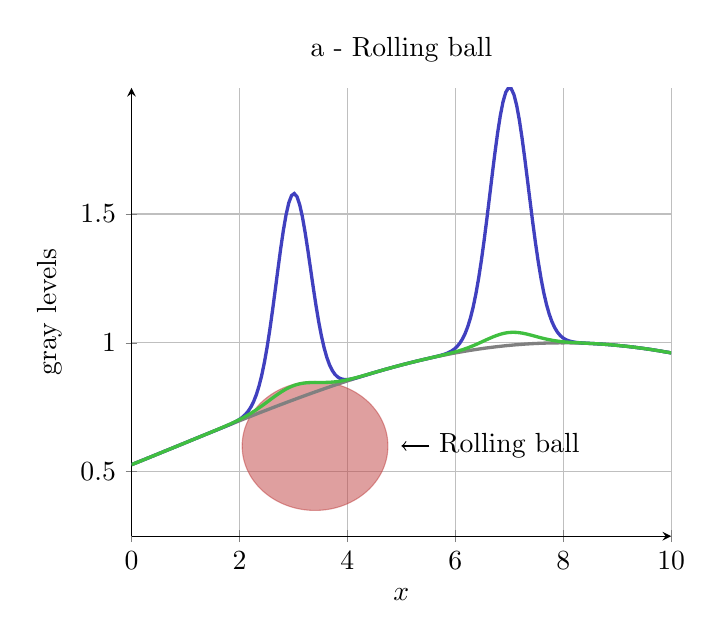
\begin{tikzpicture}
        \begin{axis}[
            axis lines=left, 
            xlabel={$x$},
            ylabel={gray levels},
            domain=0:10,
            grid=major,
            samples=200,
            ymin=0.25,
            title={a - Rolling ball}
        ]
        \draw [red!50!gray,fill,opacity=0.5] (3.4,0.6) ellipse [x radius=1.35, y radius=0.25]; 
        \node (c) at (7,0.6){Rolling ball};
        \addplot[gray,very thick] {exp(-(x-8)^2 / 100)};
        \addplot[blue!50!gray,very thick] {0.8*exp(-(x-3)^2 / 0.2)+exp(-(x-7)^2 / 0.25)+exp(-(x-8)^2 / 100)};
        \addplot[green!50!gray,very thick] {0.055*exp(-(x-3)^2 / 0.4)+0.05*exp(-(x-7)^2 / 0.4)+exp(-(x-8)^2 / 100)};
        \draw[->] (c) -- (5,0.6);
        \end{axis} 
    \end{tikzpicture}
    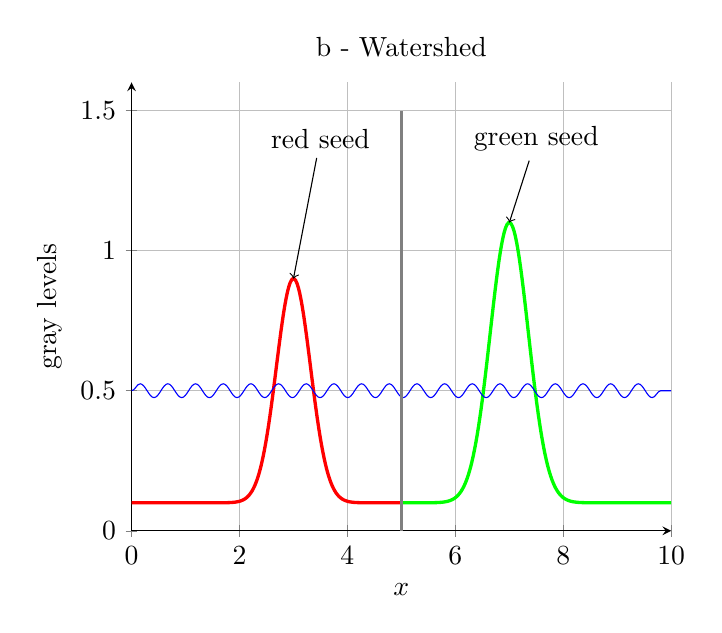
\begin{tikzpicture}
        \begin{axis}[
            axis lines=left, 
            xlabel={$x$},
            ylabel={gray levels},
            domain=0:10,
            grid=major,
            samples=200,
            ymin=0.0,
            ymax=1.6,
            title={b - Watershed}
        ]
        \addplot[red,very thick][domain=0:5] {0.1+0.8*exp(-(x-3)^2 / 0.2)+exp(-(x-7)^2 / 0.25)};
        \addplot[green,very thick][domain=5:10] {0.1+0.8*exp(-(x-3)^2 / 0.2)+exp(-(x-7)^2 / 0.25)};
        \node (a) at (3.5,1.4) {red seed};
        \node (b) at (7.5,1.4) {green seed};
        \node[circle] (ax) at (3,0.9) {};

        \draw[->] (a) -- (3,0.9);
        \draw[->] (b) -- (7,1.1);
        \draw[blue,decorate,decoration={snake}] (0,0.5) -- (10,0.5);
        \draw[gray, very thick] (5,0) -- (5,1.5);

        \end{axis} 
    \end{tikzpicture}
    \caption{Illustration of the a - rolling ball and b- watershed algorithms.}
    \label{fig:algorithm}
\end{figure}

\paragraph{Watershed} The watershed algorithm associate to seed regions pixels in the image in the order of a priority map. It can also be interpreted as flooding a landscape (see Figure~\ref{fig:algorithm}).

\subsection{Sample preparation and microscopy}

Lots of time can be saved by adjusting sample preparation and imaging to match existing  analysis tools.

\paragraph{Housekeeping labels} If possible, and when aiming at cell level statistics, include extra labels that will help identify cells location during sample preparation. A DNA stains such as DAPI and Hoescht and a plasma membrane marker such as WGA, Invitrogen's CellMask or Biotium's CellBrite can be used for example. 

\paragraph{Cell confluence} Depending on the type of analysis workflow and the cell line, high cell confluence can be counterproductive as cell will tend to grow on top of each other.

\paragraph{Dataset size} When acquiring data, have in mind the scale of the process you want to capture. If only a fraction of the cells are of interest, define multiple position instead of tiling a large field of view at high resolution will reduce the size of the dataset.





